\documentclass[12pt, a4paper, hidelinks]{article}

% Packages:
\usepackage{graphicx}                   % For figure includes
\usepackage[T1]{fontenc}                % For mixing up \textsc{} with \textbf{}
\usepackage[utf8]{inputenc}             % For scandinavian input characters(æøå)
\usepackage{amsfonts, amsmath, amssymb, amscd, amsthm} % For common mathsymbols and fonts
\usepackage[danish]{babel}              % For danish titles \usepackage{hyperref}                   % For making links and refrences
\usepackage{url}                        % Just because {~_^}
\usepackage{array}                      % ...
\usepackage[usenames, dvipsnames, svgnames, table]{xcolor}
\usepackage{tabularx, colortbl}
\usepackage{verbatim} % For entering code snippets.
\usepackage{fancyvrb} % A "fancy" verbatim (for pseudo code).
\usepackage{listings} % For boxed codesnippets, and file includes. (begin)
\usepackage{lipsum}   % For generating dummy text at this demonstration
\usepackage{float}
\usepackage{enumerate}
\usepackage{framed}  


% Basic layout:
\setlength{\textwidth}{165mm}
\setlength{\textheight}{240mm}
\setlength{\parindent}{0mm}
\setlength{\parskip}{\parsep}
\setlength{\headheight}{0mm}
\setlength{\headsep}{0mm}
\setlength{\hoffset}{-2.5mm}
\setlength{\voffset}{0mm}
\setlength{\footskip}{15mm}
\setlength{\oddsidemargin}{0mm}
\setlength{\topmargin}{0mm}
\setlength{\evensidemargin}{0mm}

% Blackboard bold
\newcommand{\NN}{\mathbb{N}}
\newcommand{\ZZ}{\mathbb{Z}}
\newcommand{\QQ}{\mathbb{Q}}
\newcommand{\RR}{\mathbb{R}}
\newcommand{\CC}{\mathbb{C}}
\newcommand{\GCD}{\operatorname{GCD}}



\newcolumntype{C}[1]{>{\centering\arraybackslash}p{#1}}

% Colors:
\definecolor{KU-red}{RGB}{144, 26, 30}

% Text Coloring:
\newcommand{\green}[1]{\textbf{\color{green}{#1}}}
\newcommand{\blue} [1]{\textbf{\color{blue} {#1}}}
\newcommand{\red}  [1]{\textbf{\color{red}  {#1}}}


% ************************* Start Document *****************
\begin{document}

% ************************* Page Header ********************
\begin{minipage}[b]{1.0\linewidth}

\includegraphics[height=30mm]{bilag/KULogo}

\vspace*{-16ex}
\begin{center}
    {\Large \bf DMA} \vspace*{1ex} \\
    {\large Ugeopgave 8} \vspace*{1ex} \\
    {\large Matti Andreas Nielsen  } \\
    {\large \today{}  }
\end{center}
\vspace*{-3pt}
{\color{KU-red}\hrule}
\end{minipage}
\vspace{2ex}

% **************** Assignment Starts Here ******************
\tableofcontents \newpage

\section{Del}
\subsection{}
Formlen for antallet af måder hvorpå man kan danne en ordnet liste af $r$ tal fra mængden $\{1,2,\dots,500\}$ når gentagelser er tilladt er
$ 500^r $ fordi selvom dét er en ordnet liste, så når gentagelser er tilladt så kan man i worst case vælge tallet 500 hver eneste gang.

Uden gentagelser kan man opskrive formlen $\frac{500!}{(500-r)!}$


\subsection{}
Lad $ n $ være længden på vores hashtable og $ 500 $ er mængden af unikke udfald eller hash værdier vores nøgle funktion $ f $ kan generer.

Så første gang vi indsætter et element så er der $ (\frac{500}{500}) = 1 \leftrightarrow 100\% $  chance for at vi ikke får en kollision,
så hvis vi f.eks vil indsætte 3 tal får vi $$ \frac{500}{500} \times \frac{499}{500} \times \frac{498}{500} $$ det kan vi prøve at sætte på samme brøkstreg
$$ \frac{500 \times 499 \times 498}{500^3} $$

Dette kan vi omskrive videre ved at bruge fakulteter til

$$ \frac{\frac{500!}{(500-n)!}}{500^n} $$

Og det er måske ikke så praktisk når man kun vil indsætte 3 tal, men hvis man skal indsætte 25 giver det mening.

f.eks 

$$ \frac{\frac{500!}{(500-30)!}}{500^{30}} = 0.41 \leftrightarrow 41\% $$ 
chance for ikke at få en kollision.


\subsection{}

Kan se på figur~\ref{fig:probability} at jeg har plottet hashfunktionen imellem 1 og 100 når den har plads til 500 hashes

\begin{figure}[htb!]
    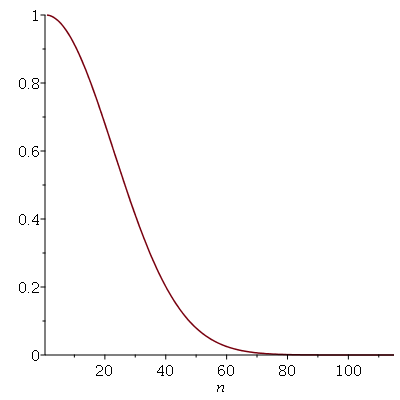
\includegraphics[width=500px, height=200px]{probability.png}
    \centering
    \caption{Sandsynligheden for at en kollision ikke forekommer i en hashtabel}
    \label{fig:probability}
\end{figure}

og det ligner at den rammer under $ 50\% $ chance for $ ikke $ at få en kollision omkring 26-28

\section{Del}

\subsection{}

Relationen $R$ på $\RR$ givet ved
\[
x R y \Longleftrightarrow x-y\in\ZZ
\]
(her er $\ZZ$ mængden af hele tal).

\begin{itemize}
\item{Symmetrisk:} 
Relationen er symmetrisk fordi
\[
xRy \Longleftrightarrow x-y\in\ZZ
\]

\[
 \Longleftrightarrow y-x\in\ZZ
\]

\[
 \Longleftrightarrow yRx
\]
\item{Refleksiv:}
Relationen er refleksiv fordi $$ x=y \implies x-y=0 \in \ZZ $$
\item{Transitiv:}
Relationen er transitiv fordi
$$ (a, b), (b,c) \in R \implies a-b \in \ZZ \land b-c \in \ZZ \implies (a-b)+(b-c) \in \ZZ \implies (a-c) \in \ZZ   $$
\end{itemize}

Vi kan derfor konkludere at relationen er en ækvivalens relation

\subsection{}

Relationen $S$ på $\RR$ givet ved
\[
xSy \Longleftrightarrow xy > 0
\]


\begin{itemize}
    \item{Symmetrisk:}
$S$ er symmetrisk pga\. det er lige meget hvilken rækkefølge man ganger i så får man det samme, dét vil sige
at alle tal som er med i relationen kan byttes om, og så vil de stadig være med i relationen.


    \item{Refleksiv:}
$S$ er ikke refleksiv fordi 
$ 0,0 \in S \land 0*0 \neq > 0 $

    \item{Transitiv:}
$S$ er transitiv, fordi 
$$ (a,b),(b,c) \in S \implies ab > 0 \land bc > 0 \implies b^{2}ac > 0 $$
Fordi $$ ab > 0 \implies b \neq 0  $$
kan vi give b en negativ eksponent, ved at gange med  $$ b^{-2}  $$
og får
$$ b^{-2}b^{2}ac > 0 \implies ac > 0 $$
\end{itemize}



\end{document}
